\documentclass[a4paper,12pt]{article}
\usepackage[utf8]{inputenc}
\usepackage{amsmath}
\usepackage{amsfonts}
\usepackage{amssymb}
\usepackage{graphicx}
\usepackage{braket}

\numberwithin{equation}{section}
\renewcommand\thesubsection{\alph{subsection}}
\newcommand{\bvp}[1]{\textbf{#1}'}
\newcommand{\bv}[1]{\textbf{#1}}

%opening
\title{Quantum I HW6}
\author{Vince Baker}

\begin{document}

\maketitle

\section{Problem 1}
The Hamiltonian of this two-level system is:
\begin{gather}
 \begin{bmatrix}
  \frac{\epsilon}{2} & \gamma\\
  \gamma    & -\frac{\epsilon}{2}
 \end{bmatrix}
\end{gather}
The energy eigenvalues are $\pm\sqrt{(\frac{\epsilon}{2})^2+\gamma^2}$.
The (unnormalized) eigenfunctions are 
$e_1=\left (1,\ \frac{\sqrt{\gamma^2+(\frac{\epsilon}{2})^2}-\frac{\epsilon}{2}}{\gamma} \right)$, 
$e_2=\left (1,\ -\frac{\sqrt{\gamma^2+(\frac{\epsilon}{2})^2}-\frac{\epsilon}{2}}{\gamma} \right)$.
The states $\ket{\uparrow}$ and $\ket{\downarrow}$ in the eigenvector basis are:
\begin{gather}
 \ket{\uparrow}=\ket{1,0}=\ket{e_1+e_2}\\
 \ket{\downarrow}=\ket{0,1}=\ket{e_1-e_2}
\end{gather}
The eigenfunctions evolve independently with an exponential phase factor. With the system starting in the $\ket{\uparrow}$ state, the time evolution of P10 and P01 is:

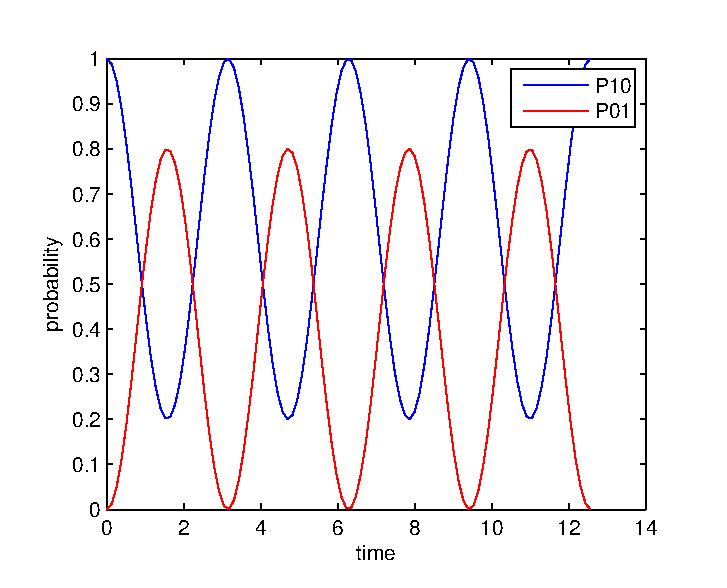
\includegraphics{p1}
\\
\section{Problem 2}


\end{document}
